% !TEX root = ../../../main.tex
% 来源：中学数学实验教材·第三册（高中数学）
% 章节：函数及其图象 / 一次函数（线性函数）
% 原始文件：4.tex，行 1365-1384
% 类型：tikz
% ---
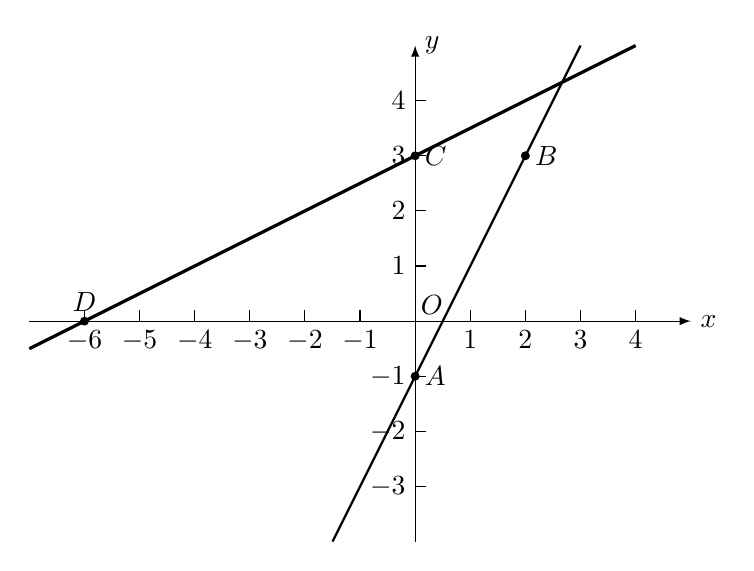
\begin{tikzpicture}[>=latex, scale=.7]
    \draw[->] (-7,0)--(5,0)node[right]{$x$};
    \draw[->] (0,-4)--(0,5)node[right]{$y$};
    \draw [domain =-1.5:3, samples=10, thick]plot(\x,{2*\x-1});
\draw [domain =-7:4, samples=10, very thick]plot(\x,{.5*\x+3});

\foreach \x in {-6,-5,...,-1,1,2,...,4}
{
    \draw (\x,0)node[below]{$\x$}--(\x,.2);
}
\foreach \x in {-3,-2,-1,1,2,3,4}
{
    \draw (0,\x)node[left]{$\x$}--(.2,\x);
}
\node at (.3,.3){$O$};
\draw (0,-1) [fill=black] circle (2pt)node[right]{$A$};
\draw (2,3) [fill=black] circle (2pt)node[right]{$B$};
\draw (0,3) [fill=black] circle (2pt)node[right]{$C$};
\draw (-6,0) [fill=black] circle (2pt)node[above]{$D$};
\end{tikzpicture}    
